\specialchapter{Bibliography}

\begin{enumerate}
\def\labelenumi{\arabic{enumi}.}
\item
  L. EULER, Vollständige Anleitung zur Algebra (=Opera Omnia (1), vol.~I, Leipzig-Berlin (Teubner), 1911).
\item
  J. L. LAGRANGE, Oeuvres, 14 volumes, Paris (Gauthier-Villars), 1867--1892.
\item
  C. F. GAUSS, Werke, 12 volumes, Göttingen, 1870--1927.
\item
  P. G. LEJEUNE-DIRICHLET, Werke, 2 volumes, Berlin (Reimer), 1889-1897.
\end{enumerate}

4 (bis). P. G. LEJEUNE-DIRICHLET, Vorlesungen über Zahlentheorie, 2te Aufl., Braunschweig (Vieweg), 1871.

\begin{enumerate}
\def\labelenumi{\arabic{enumi}.}
\setcounter{enumi}{4}
\item
  C. G. J. JACOBI, Gesammelte Werke, 7 volumes, Berlin (Reimer), 1881-1891.
\item
  G. EISENSTEIN: (a) Beweis der Reciprocitätsgesetze für die cubischen Reste in der Theorie der aus dritten Wurzeln der Einheit zusammengesetzen Zahlen, Crelle's Journal, 27 (1844), pp.~289--310; (b) Zur Theorie der quadratischen Zerfällung der Primzahlen 8n + 3, 7n + 2 und 7n + 4, Crelle's Journal, 37 (1848), pp.~97--126; (c) Über einige allgemeine Eigenschaften der Gleichung von welcher die Teilung der ganzen Lemniscate abhängt, nebst Anwendungen derselben auf die Zahlentheorie, Crelle's Journal, 39 (1850), pp.~160--179 and 224--287.
\item
  E. KUMMER: (a) Sur les nombres complexes qui sont formés avec les nombres entiers réels et les racines de l'unité, J. de Math., (1), 12 (1847), pp.~185--212; (b) Zur Theorie der complexen Zahlen, Crelle's Journal, 35 (1847), pp.~319--326; (c) Ueber die Zerlegung der aus Wurzeln der Einheit gebildeten complexen Zahlen in Primfactoren, Crelle's Journal, 35 (1847), pp.~327--367; (d) Mémoire sur les nombres complexes composés de racines de l'unité et des nombres entiers, J. de Math., (1), 16 (1851), pp.~377--498; (e) Über die allgemeinen Reciprocitätsgesetze unter den Resten und Nichtresten der Potenzen deren Grad eine Primzahl ist (Abh. der Kön. Akad. der Wiss. zu Berlin (1859), Math. Abhandl., pp.~19--159).
\item
  C. HERMITE, Oeuvres, 4 Volumes, Paris (Gauthier-Villars), 1905--1917.
\item
  L. KRONECKER, Werke, 5 volumes, Leipzig (Teubner), 1895--1930: (a) De unitatibus complexis, vol.~I, pp.~5--71 (=Inaug. Diss., Berolini, 1845); (b) Über die algebraisch auflösbaren Gleichungen I, vol.~IV, pp.~1--11 (=Monatsber. der Kön. Preuss. Akad. der Wiss., 1853, pp.~365--374); (c) Über die elliptischen Functionen für welche complexe Multiplication stattfindet vol.~IV, pp.~177--183 (=Monatsber. der Kön. Preuss. Akad. der Wiss., 1857, pp.~455--460); (d) Über die complexe Multiplication der elliptischen Functionen, vol.~IV, pp.~207--217 (=Monatsber. der Kön. Preuss. Akad. der Wiss., 1862, pp.~363--372); (e) Über die Discriminante algebraischer Functionen einer Variabeln, vol.~II, pp.~193--236 (=Crelle's Journal, 91 (1881), pp.~301--334); (f) Grundzüge einer arithmetischen Theorie der
\end{enumerate}

algebraischen Grössen, vol.~II, pp.~237--387 (=Crelle's Journal, 92 (1882), pp.~1--122).

\begin{enumerate}
\def\labelenumi{\arabic{enumi}.}
\setcounter{enumi}{9}
\tightlist
\item
  R. DEDEKIND, Gesammelte mathematische Werke, 3 volumes, Braunschweig (Vieweg), 1932: (a) Abriss einer Theorie der höheren Kongruenzen in bezug auf einen reellen Primzahl-Modulus, vol.~I, pp.~40--66 (=Crelle's Journal, 54 (1857), pp.~1--26; (b) Sur la Théorie des Nombres entiers algébriques, vol.~III, pp.~262--296 (=Bull. Sci. Math., (1), 11 (1876), pp.~278--288 and (2), 1 (1877), pp.~17--41, 69--92, 144--164, 207--248); (c) Über die Anzahl der Ideal-Klassen in den verschiedenen Ordnungen eines endlichen Körpers, vol.~I, pp.~105--157 (=Festschrift der Technischen Hochschule in Braunschweig zur Säkularfeier des Geburtstages von C. F. Gauss, Braunschweig, 1877, pp.~1--55); (d) Über den Zusammenhang zwischen der Theorie der Ideals und der Theorie der höheren Kongruenzen, vol.~I, pp.~202--230 (=Abh. Kön. Ges. Wiss. zu Göttingen, 23 (1878), pp.~1--23); (e) Über die Discriminanten endlicher Körper, vol.~I, pp.~351--396 (=Abh. Kön. Ges. Wiss. zu Göttingen, 29 (1882), pp.~1--56); (f) Über die Theorie der ganzen algebraischen Zahlen, vol.~III, pp.~1--222 (=Supplement XI von Dirichlets Vorlesungen über Zahlentheorie, 4 Aufl. (1894), pp.~434--657); (g) Zur Theorie der Ideale, vol.~II, pp.~43--48 (=Nachr. Göttingen, 1894, pp.~272--277); (h) Über eine Erweiterung des Symbols (a, b) in der Theorie der Moduln, vol.~II, pp.~59--85 (=Nachr. Göttingen, 1895, pp.~183--208).
\end{enumerate}

10 (bis). R. DEDEKIND-H. WEBER, Theorie der algebraischen Funktionen einer Veränderlichen, Crelle's Journal, 92 (1882), pp.~181--290 (=R. Dedekind, Ges. Math. Werke, vol.~I, pp.~238--349).

\begin{enumerate}
\def\labelenumi{\arabic{enumi}.}
\setcounter{enumi}{10}
\item
  E. SELLING, Ueber die idealen Primfactoren der complexen Zahlen, welche aus den Wurzeln einer beliebigen irreductiblen Gleichung rational gebildet sind, Zeitschr. für Math. und Phys., 10 (1865), pp.~17--47.
\item
  M. NOETHER, Über einen Satz aus der Theorie der algebraischen Funktionen, Math. Ann., 6 (1873), pp.~351--359.
\item
  A. BRILL-M. NOETHER, Ueber algebraischen Funktionen, Math. Ann., 7 (1874), pp.~269--310.
\item
  G. ZOLOTAREFF, Sur la théorie des nombres complexes, J. de Math. (3), 6 (1880), pp.~51--84 and 129--166.
\item
  E. NETTO, Zur Theorie der Elimination, Acta Math., 7 (1885), pp.~101-104.
\item
  D. HILBERT: (a) Über die Theorie der algebraischen Formen, Math. Ann., 36 (1890), pp.~473--534; (b) Über die vollen Invariantensysteme, Math. Ann., 42 (1893), pp.~313--373; (c) Grundzüge einer Theorie des Galoischen Zahlkörpers, Gött. Nachr., (1894), pp.~224--236; (d) Zahlbericht, Jahresber. der D. M. V., 4 (1897), pp.~175--546 (translated into French by A. Lévy and Th. Got under the title ``Théorie des corps de nombres algébriques'', Paris (Hermann), 1913).
\item
  K. WEIERSTRASS, Mathematische Werke, 7 volumes, Berlin (Mayer und Müller), 1894--1927.
\item
  K. HENSEL: (a) Über eine neue Begründung der Theorie der algebraischen Zahlen, Jahresber. der D. M. V., 6 (1899), pp.~83--88; (b) Ueber die Fundamentalgleichung und die ausserwesentlichen Diskriminantentheiler eines algebraischen Körpers, Gött. Nachr., (1897), pp.~254--260; (c) Neue Grundlagen der Arithmetik, Crelle's Journal, 127 (1902), pp.~51--84; (d) Über die arithmetische Eigenschaften der algebraischen und transzendenten Zahlen, Jahresber. der D. M. V., 14 (1905), pp.~545--558; (e) Ueber die arithmetischen Eigenschaften der Zahlen, Jahresber. der D. M. V., 16 (1907), pp.~299--319, 388--393, 474--496; (f) Theorie der algebraischen Zahlen, Leipzig (Teubner), 1908.
\item
  E. LASKER, Zur Theorie der Moduln und Ideale, Math. Ann., 60 (1905), pp.~20--116.
\item
  E. STEINITZ: (a) Algebraische Theorie der Körper, Crelle's Journal, 137 (1910), pp.~167--308; (b) Rechteckige Systeme und Moduln in algebraischen Zahlkörpern, Math. Ann. 71 (1912), pp.~328--354 and 72 (1912), pp.~297--345.
\item
  F. S. MACAULAY, On the resolution of a given modular system into primary systems including some properties of Hilbert numbers, Math. Ann., 74 (1913), pp.~66--121.
\item
  J. KÜRSCHAK, Über Limesbildung und allgemeine Körpertheorie, Crelle's Journal, 142 (1913), pp.~211--253.
\item
  A. FRAENKEL, Über die Teiler der Null und die Zerlegung von Ringen, Crelle's Journal, 145 (1914), pp.~139--176.
\item
  A. OSTROWSKI, Über einige Lösungen der Funktionalgleichung \(\phi(x)\phi(y) = \phi(x.y)\) , Acta Math., 41 (1917), pp.~271-284.
\item
  E. NOETHER: (a) Idealtheorie in Ringbereichen, Math. Ann., 83 (1921), pp.~24--66; (b) Abstrakter Aufbau der Idealtheorie in algebraischen Zahl- und Funktionenkörpern, Math. Ann., 96 (1927), pp.~26--61.
\item
  H. HASSE: (a) Ueber die Darstellbarkeit von Zahlen durch quadratischen Formen im Körper der rationalen Zahlen, Crelle's Journal, 152 (1923), pp.~129--148; (b) Ueber die Äquivalenz quadratischer Formen im Körper der rationalen Zahlen, Crelle's Journal, 152 (1923), pp.~205--224; (c) Kurt Hensels entscheidender Anstoss zur Entdeckung des Lokal-Global-Prinzips, Crelle's Journal, 209 (1960), pp.~3--4.
\item
  H. JUNG, Algebraischen Flächen, Hannover (Helwing), 1925.
\item
  H. GRELL, Beziehung zwischen den Idealen verschiedener Ringe, Math. Ann., 97 (1927), pp.~490-523.
\item
  W. KRULL: (a) Primidealketten in allgemeine Ringbereichen, Sitz. Ber. Heidelberg Akad. Wiss., 1928; (b) Allgemeine Bewertungstheorie, Crelle's Journal, 167 (1931), pp.~160--196; (c) Beiträge zur Arithmetik kommutativer Integritätsbereiche, III, Math. Zeitschr., 42 (1937), pp.~745--766; (d) Dimensionstheorie in Stellenringen, Crelle's Journal, 179 (1938), pp.~204--226; (e) Idealtheorie, Berlin (Springer), 1935.
\item
  M. H. STONE: (a) The theory of representations for Boolean algebras, Trans. Amer. Math. Soc., 40 (1936), pp.~37-111; (b) Applications of the theory of Boolean rings to general topology, Trans. Amer. Math. Soc., 41 (1937), pp.~375-481.
\item
  B. L. van der WAERDEN, Moderne Algebra, vol.~II, Berlin (Springer), 1931.
\item
  C. CHEVALLEY: (a) Généralisation de la théorie du corps de classes pour les extensions infinies, J. de Math., (9), 15 (1936), pp.~359--371; (b) On the theory of local rings, Ann. of Math., 44 (1943), pp.~690--708.
\item
  O. ZARISKI: (a) The compactness of the Riemann manifold of an abstract field of algebraic functions, Bull. Amer. Math. Soc., 50 (1944), pp.~683--691; (b) Generalized semi-local rings, Summa Bras. Math., 1 (1946), pp.~169--195.
\item
  N. JACOBSON, A topology for the set of primitive ideals in an arbitrary ring, Proc. Nat. Acad. Sci. U.S.A., 31 (1945), pp.~333--338.
\item
  I. COHEN-A.SEIDENBERG, Prime ideals and integral independence, Bull. Amer. Math. Soc., 52 (1946), pp.~252--261.
\item
  P. SAMUEL, La notion de multiplicité en Algèbre et en Géométrie algébrique, J. de Math., (9), 30 (1951), pp.~159--274.
\item
  A. WEIL, Fibre-spaces in Algebraic Geometry (Notes by A. Wallace), Chicago Univ., 1952.
\item
  J. P. SERRE: (a) Faisceaux algébriques cohérents, Ann. of Math., 61 (1955), pp.~197--278; (b) Géométrie algébrique et géométrie analytique, Ann. Inst. Fourier, 6 (1956), pp.~1--42.
\item
  A. GROTHENDIECK, Éléments de géométrie algébrique, Publ. math. Inst. Htes Et. Scient., 1960.
\end{enumerate}

\specialchapter{Index of notation}

The reference numbers indicate the chapter, section and sub-section (or exercise) in that order.

\(l_{E}\) (E a set), U.V, UV (U, V additive subgroups), \(a^{0}\) (a an ideal): Preliminary conventions of Chapter I

E:F:I.2.10

\(\mathbf{A}[\mathbf{S}^{-1}], a / s\) (A a ring, S a subset of \(\mathbf{A}\) , \(a \in \mathbf{A}\) , \(s\) a product of elements of \(\mathbf{S}\) ): II.2.1 \(i_{\mathbf{A}}^{\mathbf{S}}\) : II.2.1

\(\mathbf{S}^{-1}\mathbf{A},\mathbf{A}_{p}\) (S a multiplicative subset, p a prime ideal): II.2.1

\(\mathbf{M}[\mathbf{S}^{-1}], m / s, i_{\mathbf{M}}^{\mathbf{S}}\) (M an A-module, S a subset of \(\mathbf{A}\) , \(m \in \mathbf{M}\) , \(s\) a product of elements of \(\mathbf{S}\) ): II.2.2

\(S^{-1}M, M_{p}\) (M an A-module, S a multiplicative subset of A, p a prime ideal of A): II.2.2

\(\mathbf{S}^{-1}u, u_{p}\) ( \(u\) an A-module homomorphism): II.2.2

r(a) (a an ideal): II.2.6

\(\mathbf{V}(\mathbf{M}), \mathbf{V}(f) (\mathbf{M}\) a subset of the ring \(\mathbf{A}, f \in \mathbf{A})\) : II.4.3

\(\operatorname {Spec}(\mathbf{A})\) : II.4.3

\(\mathbf{X}_f\) ( \(f \in \mathbf{A}\) , \(\mathbf{X} = \operatorname{Spec}(\mathbf{A})\) ): II.4.3

\(\Im (\mathbf{Y})\) (Y a subset of \(\operatorname {Spec}(\mathbf{A}))\) : II.4.3

\(^{a}h\) (h a ring homomorphism): II.4.3

Supp(M) (M an A-module): II.4.4

\(\mathbf{A}_f, \mathbf{M}_f, u_f\) (A a ring, M an A-module, \(u\) an A-homomorphism, \(f \in \mathbf{A}\) ): II.5.1

\(\mathbf{rg}_{\mathfrak{p}}(\mathbf{P})\) (P a projective module): II.5.3

rg(P) (P a projective module): II.5.3

\(P(A)\) , cl(M) (A a ring, M a projective A-module of rank 1): II.5.4

\(\operatorname{det}(u), \chi_u\) ( \(u\) an endomorphism of a projective module of rank \(n\) ): II.5. Ex. 9

\(\mathbf{A}^{(d)}, \mathbf{M}^{(d,k)}, \mathbf{M}^{(d)}\) (A a graded ring, M a graded A-module): III.1.3

\(A_{(p)}, M_{(p)}\) (A a graded ring, p a graded prime ideal of A, M a graded A-module): III.1.4

\(\mathbf{gr}_n(\mathbf{G}), \mathbf{gr}(\mathbf{G})\) (G a filtered group): III.2.3

gr(h) (h a homomorphism compatible with the filtrations): III.2.4

\(\mathbf{Z}_n\) ( \(n\) an integer \(>1\) ): III.2.12

\(\hat{\mathbf{Z}}\) : III.2.13

\(\mathrm{A}\{\mathrm{X}_1,\dots ,\mathrm{X}_p\}\) (A a linearly topologized ring): III.4.2

\(f(b_{1},\ldots ,b_{p})\) (f a restricted formal power series): III.4.2

\(\mathbf{f} \circ \mathbf{g}, M_{t}, M_{t}(\mathbf{X}), J_{t}, J_{t}(\mathbf{X}), \mathbf{X}, \mathbf{1}_{n}\) ( \(\mathbf{f}, \mathbf{g}\) systems of formal power series, \(\mathbf{g}\) without constant term): III.4.4

\(\mathbf{f}(\mathbf{x})\) (f a system of formal power series, \(\mathbf{x}\) a system of topological nilpotent elements): III.4.5

\(\mathfrak{m}^{\times n}\) (m an ideal): III.4.5

\(\operatorname{Ass}_{\mathbf{A}}(\mathbf{M}), \operatorname{Ass}(\mathbf{M})\) (M an A-module): IV.1.1

\(\mathbf{Ass}_f(\mathbf{M})\) : IV.1. Ex. 17

\(\mathbf{A}^{\mathcal{G}}\) (A an algebra, \(\mathcal{G}\) a group operating on A): V.1.9

\(\mathcal{G}^{\mathrm{Z}}(\mathfrak{p}^{\prime}), \mathcal{G}^{\mathrm{Z}}, \mathrm{A}^{\mathrm{Z}}(\mathfrak{p}^{\prime}), \mathrm{A}^{\mathrm{Z}}\) (G a group operating on a ring \(\mathrm{A}'\) , \(\mathfrak{p}'\) a prime ideal of \(\mathrm{A}'\) ): V.2.2

\(\mathcal{G}^{\mathrm{T}}(\mathfrak{p}')\) , \(\mathcal{G}^{\mathrm{T}}\) , \(\mathbf{A}^{\mathrm{T}}(\mathfrak{p}')\) , \(\mathbf{A}^{\mathrm{T}}\) ( \(\mathcal{G}\) a group operating on a ring \(\mathbf{A}'\) , \(\mathfrak{p}'\) a prime ideal of \(\mathbf{A}'\) ): V.2.2

\(\mathbf{K}^{\mathrm{Z}}(\mathfrak{p}')\) , \(\mathbf{K}^{\mathrm{Z}}\) , \(\mathbf{K}^{\mathrm{T}}(\mathfrak{p}')\) , \(\mathbf{K}^{\mathrm{T}}\) (K the field of fractions of an integrally closed domain

A, \(p'\) a prime ideal of the integral closure of A in a quasi-Galois extension of K): V.2.3

\(\mathbf{Y}^{\mathbf{p}}\) (where \(\mathbf{p} = (p_1, \ldots, p_m)\) , the \(p_i\) being integers \(\geqslant 0\) ): V.3.1

\(\mathfrak{m}(\mathbf{A}), \kappa(\mathbf{A}), \mathrm{U}(\mathbf{A})\) (A a local ring): VI

\(\tilde{\mathbf{K}},\infty :\mathbf{VI}.2.1\)

+∞: VI.3.1

\(\Gamma_{\mathbf{A}}, v_{\mathbf{A}}\) : VI.3.2

\(\mathfrak{a}(\mathbf{M})\) (M a major set): VI.3.5

\(h(\mathbf{G})\) (G a totally ordered group): VI.4.4

\(\mathcal{T}_v\) ( \(v\) a valuation): VI.5.2

\(e(v^{\prime} / v), e(\mathbf{A}^{\prime} / \mathbf{A}), e(\mathbf{L} / \mathbf{K})\) : VI.8.1

\(f(v^{\prime} / v),f(\mathbf{A}^{\prime} / \mathbf{A}),f(\mathbf{L} / \mathbf{K})\) : VI.8.1

\(\varepsilon (\mathrm{G},\mathrm{H})\) (G a totally ordered group, H a subgroup of G of finite index): VI.8.4

\(\varepsilon(v'/v)\) ( \(v\) a valuation, \(v'\) an extension of \(v\) ): VI.8.4

mod(x), mod\_K(x) (K a non-discrete locally compact field, x ∈ K): VI.9.1

\(r(\mathbf{G})\) (rational rank of a commutative group): VI.10.2

\(d(\mathbf{K}' / \mathbf{K}), s(v' / v), r(v' / v)\) (v a valuation on \(\mathbf{K}\) , \(v'\) an extension of \(v\) to a transcendental extension \(\mathbf{K}'\) of \(\mathbf{K}\) ): VI.10.3

I(A), D(A) (A an integral domain): VII.1.1

\(\mathfrak{a} \prec \mathfrak{b}\) , \(\operatorname{div}(\mathfrak{a})\) , \(\operatorname{div}(x)\) ( \(\mathfrak{a}\) , \(\mathfrak{b}\) fractional ideals, \(x\) an element of the field of fractions): VII.1.1

\(\tilde{\mathfrak{a}}\) (a a fractional ideal): VII.1.1

\(d_{1} \leqslant d_{2}\) ( \(d_{1}, d_{2}\) divisors): VII.1.1

b: a (a, b fractional ideals): VII.1.1

J(A) (A an integral domain): VII.1.2

P(A) (A a Krull domain): VII.1.3

\(\mathfrak{p}^{(n)}\) (p a divisorial prime ideal): VII.1.4

\(v_{p}\) (p a prime ideal of height 1 in a Krull domain): VII.1.10

\(\mathbf{F}(\mathbf{A}), \mathbf{C}(\mathbf{A})\) (A a Krull domain): VII.1.10

\(e(\mathfrak{P}/\mathfrak{p})\) \((\mathfrak{p}\in\mathrm{P}(\mathrm{A}),\;\mathfrak{P}\in\mathrm{P}(\mathrm{B}),\;\mathrm{A}\;\text{and}\;\mathrm{B}\;\text{Krull domains},\;\mathrm{A}\subset\mathrm{B},\;\mathfrak{P}\cap\mathrm{A}=\mathfrak{p}):\) VII.1.10

\(i\) (homomorphism from \(\mathbf{D}(\mathbf{A})\) to \(\mathbf{D}(\mathbf{B})\) , or of \(\mathbf{C}(\mathbf{A})\) to \(\mathbf{C}(\mathbf{B}))\) : VII.1.10

\(\bar{i}\) (homomorphism from \(\mathbf{C}(\mathbf{A})\) to \(\mathbf{C}(\mathbf{B}))\) : VII.1.10

\(A, A_{0}, \Delta(K)\) (rings of restricted adèles): VII.2.4

\(\mathfrak{P}^*, \mathfrak{P}^*(\mathbf{A})\) (A an integral domain): VII.3.2

M* (dual lattice of a lattice M): VII.4.2

\(l_{\mathfrak{p}}(\mathrm{T}), \chi (\mathrm{T})\) (T a torsion A-module, \(\mathfrak{p}\) a prime ideal of height 1): VII.4.5

\(\pmb {F}(\mathbf{A}),\pmb{T}(\mathbf{A}),\mathrm{cl}(\mathbf{M}):\) VII.4.5

\(\chi (\mathbf{M},\mathbf{M}^{\prime})\) (M, \(\mathbf{M}'\) lattices):VII.4.6

\(c(d)\) ( \(d\) a divisor):VII.4.7

\(c(\mathbf{M}), r(\mathbf{M}), \gamma(\mathbf{M})\) (M a lattice): VII.4.7

\(\mathfrak{P}|\mathfrak{p},e_{\mathfrak{P} / \mathfrak{p}},f_{\mathfrak{P} / \mathfrak{p}},f(\mathfrak{P} / \mathfrak{p})\) (A \(\subset\) B Krull domains such that B is a finite A-algebra

\(\mathfrak{p} \in \mathrm{P}(\mathbf{A}), \mathfrak{P} \in \mathrm{P}(\mathbf{B}), \mathfrak{P} \cap \mathbf{A} = \mathfrak{p}\) : VII.4.8

\(\mathbf{N}_{\mathbf{B} / \mathbf{A}},\mathbf{N},i_{\mathbf{B} / \mathbf{A}}\) :VII.4.8

\specialchapter{Index of terminology}

The reference numbers indicate the chapter, section and sub-section (or exercise) in that order.

Adèle, restricted, principal restricted adèle: VII.2.4

m-adic filtration: III.2.1

--- topology: III.2.5

\(n\) -adic integers: III.2.12

Algebra, Azumaya: II.1.7

--- finitely generated: III.1.1

--- integral, finite, over a ring: V.1.1

Algebraic closure of a field in an algebra: V.1.2

Algebraically closed field in an algebra: V.1.2

--- dependent, independent, elements: III.1.1

--- free, related, family: III.1.1

Almost all \(\mathfrak{p} \in \mathbf{P}(\mathbf{A})\) (property valid for): VII.4.3

--- nilpotent endomorphism: IV.1.4

Approximation theorem for absolute values: VI.7.3

--- theorem for valuations: VI.7.2

Artin-Rees Lemma: III.3.1

Associated (filtered module) with a graded module: III.2.1

--- (filtered ring) with a graded ring: III.2.1

--- (filtration) with a graduation: III.2.1

--- (graded homomorphism) with a homomorphism compatible with filtrations: III.2.4

--- (graded module) with a filtered module: III.2.3

--- (graded ring) with a filtered ring: III.2.3

--- (mapping) with a ring homomorphism: II.4.3

--- (prime ideal) with a module: IV.1.1

--- ring, place, valuation: VI.3.3

Canonical decomposition of a place: VI.2.3

--- factorization of a valuation: VI.3.2

---homomorphism of the decomposition group of a prime ideal \(\mathfrak{p}'\) of A' into

the automorphism group of A'/p': V.2.2

Class, divisor, attached to a finitely generated module: VII.4.7

Classes, divisor (monoid of): VII.1.2

Closure, algebraic, of a field in an algebra: V.1.2

--- integral, of an integral domain: V.1.2

--- integral, of a ring in an algebra: V.1.2

Commutative diagram: I.1.2

Compatible (filtration) with a ring structure, module structure: III.2.1

--- (homomorphism) with filtrations: III.2.4

Complete system of extensions of a valuation: VI.8.2

Completely integrally closed domain: V.1.4

Component, irreducible (of a topological space): II.4.1

Conditions, Hensel's: III.4.5

Conductor of a submodule: V.1.5

Content of a polynomial over a pseudo-Bezoutian domain: VII.1.Ex.23

--- of a torsion module: VII.4.5

Criterion, Eisenstein's irreducibility: VII.3.Ex.20

Decomposition, canonical, of a place: VI.2.3

--- complete, of a prime ideal: V.2.2

--- field of a prime ideal: V.2.2

--- group, ring, of a prime ideal: V.2.2

--- of an ideal in a Dedekind domain into prime factors: VII.2.3

--- primary: IV.2.2 and Ex.20

--- reduced primary: IV.2.3 and Ex.20

Decreasing filtration: III.2.1

Dedekind domain: VII.2.1

Defined (topology) by a filtration: III.2.5

Defining ideal: III.3.2

Degree, residue class, of one valuation over another: VI.8.1

Dependence, integral (equation of): V.1.1

Derived (module filtration) from a ring filtration: III.2.1

Diagram, commutative: I.1.2

--- snake: I.1.4

Discrete filtration: III.2.1

--- valuation: VI.3.6

Distinguished polynomial: VII.3.8

Divisor, principal divisor: VII.1.1

--- determinantal: VII.4.Ex.11

--- finitely generated: VII.1.Ex.11

Divisorial fractional ideal: VII.1.1

Divisors, equivalent: VII.1.2

Domain, Bezoutian (or Bezout): VII.1.Ex.20

--- completely integrally closed: V.1.4

--- Dedekind: VII.2.1

--- factorial: VII.3.1

--- integrally closed: V.1.2

--- integrally closed, of finite character: VII.1.Ex.25, 26 and 28

--- integrally Noetherian: V.3.Ex.6

--- Krull: VII.1.3

--- local integral, of dimension 1: VI.4.Ex.7

--- Prüferian (or Prüfer): VII.2.Ex.12

--- pseudo-Bezoutian: VII.1.Ex.21

--- pseudo-principal: VII.1.Ex.21

--- pseudo-Prüferian: VII.2.Ex.19

--- regularly integrally closed: VII.1.Ex.30

Dominating (local ring) a local ring: VI.1.1

Dual, algebraic toric, of a module: VI.5.Ex.9

--- lattice: VII.4.2

--- topological toric: VI.5.Ex.10

Element, topologically nilpotent: III.4.3

Elements, algebraically dependent, independent: III.1.1

--- strongly relatively prime: III.4.1

Endomorphism, almost nilpotent: IV.1.4

Equivalent divisors: VII.1.2

--- valuations: VI.3.2

Essential graded ideal: III.1.4

--- valuations: VII.1.4

Euclidean ordered field: VI.2.Ex.4

Exhaustive filtration: III.2.1

Extension, quasi-Galois: V.2.2

Factor, invariant: VII.4.Ex.11 and 14

Factorial domain: VII.3.1

Factorization, canonical, of a valuation: VI.3.2

Faithfully flat module: I.3.1

Family, algebraically free, related: III.1.1

--- formally free: III.2.9

Field, algebraically closed in an algebra: V.1.2

--- decomposition: V.2.3

--- projective: VI.2.1

--- residue, of a local ring: II.3.1

Field, residue, of a place: VI.2.3

--- residue, of a valuation: VI.3.2

--- value, of a place: VI.2.2

Filtered group, ring, module: III.2.1

Filtration, m-adic: III.2.1

--- associated with a graduation: III.2.1

--- compatible with a ring structure, module structure: III.2.1

--- discrete: III.2.5

--- m-good: III.3.1

--- increasing, decreasing, separated, exhaustive: III.2.1

--- induced, product, quotient: III.2.1

--- module, derived from a ring filtration: III.2.1

--- trivial: III.2

Finite algebra over a ring: V.1.1

--- (place) at an element: VI.2.2

Finitely generated algebra: III.1.1

Finitely presented: I.2.8

Flat for M, M-flat (module): I.2.2

--- module: I.2.3

Formally free family: III.2.9

Fractional ideal: VII.1.1

Function, order: III.2.2

Gaussian integer: V.1.1

Gauss's lemma: VII.3.5

Gelfand-Mazur Theorem: VI.6.4.

Generated by a subset (multiplicative subset): II.2.1

Generators, formal system of: III.2.9

m-good filtration: III.3.1

Group, decomposition: V.2.2

--- filtered: III.2.1

--- inertia: V.2.2

--- of classes of invertible modules: II.5.7

--- of operators, locally finite: V.1.9

--- operating on a ring: V.1.9

--- order, of a valuation: VI.3.2

--- ordered, of height n, of height +∞: VI.4.4

Height \(\leqslant 1\) (prime ideal of): VII.1.6

--- of an ordered group, of a valuation: VI.4.4

Henselian ring: III.4.Ex.3

Hensel's conditions: III.4.5

--- Theorem: III.4.3

Homomorphism, canonical, of the decomposition group of a prime ideal \(p'\)

--- from A' to the automorphism group of A'/p': V.2.2

--- compatible with filtrations: III.2.4

--- graded, associated with a homomorphism compatible with filtrations: III.2.4

--- local: II.3.1

--- pseudo-injective, pseudo-surjective, pseudo-zero, pseudo-bijective: VII.4.4

Ideal, determinantal: VII.4.Ex.10 and 14

--- essential graded: III.1.4

--- immersed prime: IV.2.3

--- integral, fractional ideal: VII.1.1

--- invertible fractional: II.5.7

--- lying above an ideal: V.2.1

--- minimal prime: II.2.6

--- of a place: VI.2.3

--- of a valuation: VI.3.2

---prime:II.1.1

--- prime, associated with a module: IV.1.1

--- prime, decomposing completely: V.2.2

--- prime, of height ≤1: VII.1.6

--- primary, p-primary: IV.2.1 and Ex.20

--- unramified: V.2.Ex.18 and 19

Ideally Hausdorff module: III.5.1

Ideals, relatively prime: II.1.2

Identity, Cauchy's: VII.3.Ex.18

Immersed prime ideal: IV.2.3

Improper valuation: VI.3.1

Increasing filtration: III.2.1

Independent valuation rings: VI.7.2

--- valuations: VI.7.2

Index, initial, of a subgroup of an ordered group, initial ramification index of a valuation: VI.8.4

---ramification: VI.8.1

Induced filtration: III.2.1

Induction, Noetherian (principle of): II.4.2

Inertia field: V.2.3

--- ring, group: V.2.2

Initial ramification index: VI.8.4

Integer, algebraic: V.1.1

--- Gaussian: V.1.1

--- over a ring: V.1.1

\begin{Shaded}
\begin{Highlighting}[]
\NormalTok{Integers, n{-}adic: III.2.12}
\NormalTok{Integral algebra over a ring: V.1.1}
\NormalTok{— closure: V.1.2}
\NormalTok{— ideal: VII.1.1}
\NormalTok{Integrally closed domain: V.1.2}
\NormalTok{— closed in an algebra (ring): V.1.2}
\NormalTok{Invariant, relative, of one lattice with respect to another: VII.4.6}
\NormalTok{Invertible fractional ideal: II.5.7}
\NormalTok{— submodule: II.5.6}
\NormalTok{Irreducible component: II.4.1}
\NormalTok{— set: II.4.1}
\NormalTok{— space: II.4.1}
\NormalTok{Isolated subgroup: VI.4.2}
\NormalTok{Jacobson ring: V.3.4}
\NormalTok{Krull{-}Akizuki Theorem: VII.3.5}
\NormalTok{Krull domain: VII.1.3}
\NormalTok{Krull\textquotesingle{}s Theorem: III.3.2}
\NormalTok{Laskerian module: IV.2.Ex.23}
\NormalTok{Lattice: VII.4.1}
\NormalTok{— dual: VII.4.2}
\NormalTok{— reflexive: VII.4.2}
\NormalTok{Lemma, Artin{-}Rees: III.3.1}
\NormalTok{— Gauss\textquotesingle{}s: VII.3.5}
\NormalTok{— normalization: V.3.1}
\NormalTok{Linearly topologized ring: III.4.2}
\NormalTok{Local homomorphism: II.3.1}
\NormalTok{— ring: II.3.1}
\NormalTok{Locally finite group of operators: V.1.9}
\NormalTok{Lying above (ideal) an ideal: V.2.1}
\NormalTok{Major set: VI.3.5}
\NormalTok{Mapping, continuous, associated with a ring homomorphism: II.4.3}
\NormalTok{Minimal polynomial: V.1.3}
\NormalTok{— prime ideal: II.2.6}
\NormalTok{Module, coherent: I.2.Ex.11}
\NormalTok{— faithfully flat: I.3.1}
\NormalTok{— filtered: III.2.1}
\NormalTok{— filtered, associated with a graded module: III.2.1}
\NormalTok{— finitely presented: I.2.8}
\NormalTok{— flat: I.2.3}
\NormalTok{— flat for M, M{-}flat: I.2.2}
\end{Highlighting}
\end{Shaded}

\begin{Shaded}
\begin{Highlighting}[]
\NormalTok{— minimal: V.1.3}
\end{Highlighting}
\end{Shaded}

Module graded, associated with a filtered module: III.2.3

--- ideally Hausdorff: III.5.1

--- of fractions defined by a subset of a ring: II.2.2

--- projective, of rank n: II.5.3

--- pseudo-coherent: I.2.Ex.11

--- pseudo-zero: VII.4.4

Monoid, divisor class: VII.1.2

Morphism for laws of composition not everywhere defined: VI.2.1

Multiplicative subset: II.2.1

Nilradical of a ring: II.2.6

Noetherian space: II.4.2

Non-degenerate submodule: II.5.5

Normalization lemma: V.3.1

Normed discrete valuation: VI.3.6

Nullstellensatz: V.3.3

Order group of a valuation: VI.3.2

--- of an element for a valuation: VI.3.2

--- reduced, of a formal power series: VII.3.8

Ordered pair of rings with the linear extension property: I.3.7

Ostrowski's theorem: VI.6.4

Place, finite at \(x\) : VI.2.2

--- trivial: VI.2.2

Point, generic, of an irreducible space: II.4.Ex.2

Polygon, Newton: VI.4.Ex.11

Polynomial, distinguished: VII.3.8

Preparation theorem: VII.3.8

Presentation of a module, --- finite: I.2.8

\(n\) -presentation: I.2.Ex.6

Presented, finitely (module): I.2.8

Primary decomposition: IV.2.2 and Ex.20

--- p-primary, ideal, submodule: IV.2.1 and Ex.20

Prime ideal: II.1.1

--- spectrum: II.4.3

Principal divisor: VII.1.1

--- restricted adèle: VII.2.4

Principle of Noetherian induction: II.4.2

Product filtration: III.2.1

Projective field: VI.2.1

Pseudo-injective, pseudo-surjective, pseudo-zero, pseudo-bijective (homomorphism): VII.4.4

Pseudo-isomorphism: VII.4.4

Pseudo-zero module: VII.4.4

Quasi-Galois extension: V.2.2

Quotient filtration: III.2.1

Radical of an ideal: II.2.6 Rank at p of a projective module: II.5.3 --- of a projective module: II.5.3 --- rational, of a commutative group: VI.10.2 --- residue: VI.8.5 Rational rank of a commutative group: VI.10.2 Reduced order: VII.3.8 --- primary decomposition: IV.2.3 --- ring: II.2.6 --- series: VII.3.8 Reflexive lattice: VII.4.2 Related local rings: VI.1.Ex.1 Relatively prime ideals: II.1.2 Representative system of extremal elements: VII.3.3 Residue class degree of a valuation: VI.8.1 --- field: II.3.1 --- rank of a valuation: VI.8.5 Resolution, finite free, of a module: VII.4.7 Restricted adèle: VII.2.4 --- formal power series: III.4.2 Ring, absolutely flat: I.2.Ex.17 --- coherent (left, right): I.2.Ex.17 --- decomposition: V.2.2 --- filtered: III.2.1 --- filtered, associated with a graded ring: III.2.1 --- graded, associated with a filtered ring: III.2.3 --- inertia: V.2.2 --- integrally closed in an algebra: V.1.2 --- Jacobson: V.3.4 --- linearly topologized: III.4.2 --- local: II.3.1 --- local, dominating a local ring: VI.1.1 --- local, of A at p, of p (p a prime ideal): II.3.1 --- of a place: VI.2.3 --- of a valuation: VI.3.2

Ring of fractions defined by a subset of a ring: II.2.1

--- reduced: II.2.6

--- semi-local: II.3.5

--- total, of fractions: II.2.1

--- unramified: V.2.Ex.19

--- valuation, valuation ring of a field: VI.1.1

--- Zariski: III.3.3

Rings, independent valuation: VI.7.2

Saturation of a submodule with respect to a multiplicative subset (with respect

to a prime ideal): II.2.4

Semi-local ring: II.3.5

Series, reduced: VII.3.8

--- restricted formal power: III.4.2

Set, irreducible: II.4.1

--- major, in a totally ordered group: VI.3.5

Space, irreducible: II.4.1

--- Noetherian: II.4.2

Special topology: II.4.3

Spectrum, prime, of a ring: II.4.3

Strongly Laskerian module: IV.2.Ex.28

--- primary submodule: IV.2.Ex.27

--- relatively prime elements: III.4.1

Subgroup, isolated, of an ordered group: VI.4.2

Submodule, invertible: II.5.6

--- non-degenerate: II.5.5

--- primary, p-primary: IV.2.1

Subset, multiplicative, of a ring: II.2.1

--- multiplicative, generated by a subset: II.2.1

--- saturated multiplicative: II.2.Ex.1

Support of a module: II.4.4

System, complete, of extensions of a valuation: VI.8.2

--- formal, of generators: III.2.9

--- representative, of extremal elements: VII.3.3

Theorem, approximation, for absolute values: VI.7.3

--- approximation, for valuations: VI.7.2

--- Gelfand-Mazur: VI.6.4

--- Hensel's: III.4.3

--- Hilbert's zeros (Nullstellensatz): V.3.3

--- Krull's: III.3.1

--- Krull-Akizuki: VII.3.5

--- Ostrowski's: VI.6.3

Theorem, preparation: VII.3.8

--- Stickelberger's: VI.8.Ex.18

--- Zariski's Principal: V.3.Ex.7

Topologically nilpotent element: III.4.3

Topology defined by a filtration: III.2.5

--- spectral: II.4.3

--- Zariski: II.4.3

Transporter: I.2.10

Trivial filtration: III.2.1

--- place: VI.2.2

Ultrametric absolute value: VI.6.1

Uniformizer for a discrete valuation: VI.3.6

Unramified valuation: VI.8.1

Valuation, valuation of an element x: VI.3.1 and 2

--- discrete, normed discrete valuation: VI.3.6

--- essential: VII.1.4 and Ex.26

--- improper: VI.3.1

---ring: VI.1.1

--- unramified: VI.8.1

Valuations, equivalent: VI.3.2

--- independent: VI.7.2

Value field of a place: VI.2.2

--- ultrametric absolute: VI.6.1

Weakly associated (prime ideal) with a module: IV.1.Ex.17

Zariski, ring: III.3.3

--- topology: II.4.3

\specialchapter{Table of implications}

\pandocbounded{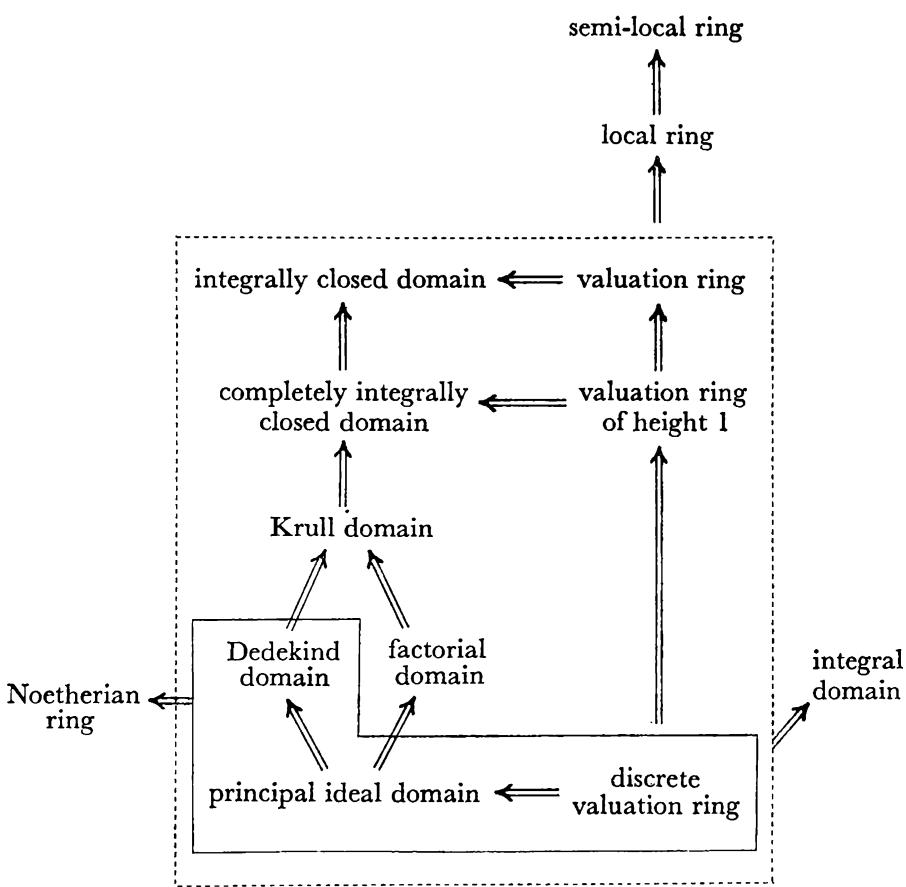
\includegraphics[keepaspectratio]{images/part004_39dc4b31.jpg}}

In the case of Noetherian rings this table reduces to the following:

\pandocbounded{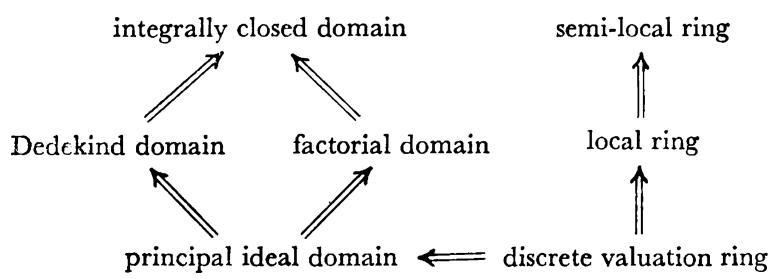
\includegraphics[keepaspectratio]{images/part004_7c195a13.jpg}}

\specialchapter{Table of invariances --- I}

In this table and the following, each row corresponds to a property a ring may possess and each column to a ring derived from the ring A (p denoting a prime ideal of A, S a multiplicative subset of A not containing 0 and A' the integral closure of A in a finite algebraic extension L of the field of fractions K of A). The ring A is assumed to possess the property indicated in the row; the word ``yes'' (resp. ``no'', ``?'') at the intersection of this row and a column means that it is true (resp. false, still unknown) that every ring constructed from A by the process indicated by the column has the property indicated by the row.

The references indicate the place in this Book or the Book Algebra where the result in question is proved, and similarly for the two following works where results not mentioned in the text or in the exercises are concerned:

\begin{enumerate}
\def\labelenumi{(\arabic{enumi})}
\item
  A. GROTHENDIECK, Éléments de géométrie algébrique, Chapter IV (Publ. Inst. Htes Études Scient., nos. 20 and 24, 1964).
\item
  M. NAGATA, Local rings, Interscience (New York), 1962.
\end{enumerate}

A/p

\(S^{-1}A\)

A{[}X{]}

A{[}{[}X{]}{]}

A'

A a principal ideal domain

YES

YES

NO Alg. VII, § 1, Ex. 1

NO

NO Alg. VII, § 1, Ex. 12

A a Dedekind domain

YES

YES

NO Alg. VII, § 1, Ex. 1

NO VII, § 1, Ex. 9

YES VII, § 2, Cor. 2 to Prop. 9)

A a factorial domain

NO V, § 1, Ex. 9

YES VII, § 3, Prop. 3

YES VII, § 3, Th. 2

NO VII, § 3, Ex. 9

NO Alg. VII, § 1, Ex. 12

A a Noetherian integrally closed domain

NO V, § 1, Ex. 9

YES V, § 1, Cor. 1 to Prop. 16

YES V, § 1, Cor. 1 to Prop. 13

YES V, § 1, Prop. 14

? (YES if L is separable; V, § 1, Cor. 1 to Prop. 18)

A a field or a discrete valuation ring

YES VI, § 3, no. 6

YES VI, § 3, no. 6

NO Alg. VII, § 1, Ex. 1

NO VII, § 1, Ex. 9

NO V, § 2, Ex. 6

A a field or a valuation ring of height 1

YES VI, § 4

YES VI, § 4, Prop. 1

NO Alg. VII, § 1, Ex. 1

NO VII, § 1, Ex. 9

NO V, § 2, Ex. 6

A a valuation ring

YES VI, § 1, Th. 1

YES VI, § 1, Th. 1

NO Alg. VII, § 1, Ex. 1

NO VII, § 1, Ex. 9

NO V, § 2, Ex. 6

A a complete valuation ring

YES VI, § 5, Prop. 1

YES VI, § 7, Prop. 3

NO Alg. VII, § 1, Ex. 1

NO VII, § 1, Ex. 9

NO V, § 2, Ex. 6

A a Krull domain

NO V, § 1, Ex. 9

YES VII, § 1, Prop. 6

YES VII, § 1, Prop. 13

YES VII, § 1, Ex. 9

YES VII, § 1, Prop. 12

\specialchapter{Table of invariances --- II}

In this table a denotes an ideal of A distinct from A, S a multiplicative subset of A and A' the integral closure of A which is assumed to be an integral domain.

A/a

\(S^{-1}A\)

A{[}X{]}

A{[}{[}X{]}{]}

A\textquotesingle{}

A local

YES

NO II, § 2, Prop. 11

NO

YES Alg. IV, § 5, Prop. 4

NO V, § 2, Ex. 20

A local and complete

? YES if A is Noetherian (III, § 3, Prop. 6)

NO II, § 2, Prop. 11

NO

YES III, § 2, Prop. 6

? YES if A is Noetherian (1)

A semi-local

YES

NO IV, § 2, Ex. 23(c)

NO

YES Alg. IV, § 5, Prop. 4

? YES if A is Noetherian V, § 2, Ex. 7

A semi-local and complete

? YES if A is Noetherian (III, § 3, Prop. 6)

NO IV, § 2, Ex. 23(c)

NO

YES III, § 2, Prop. 6

A Noetherian

YES Alg. VIII, § 2, Prop. 6

YES II, § 2, Cor. 2 to Prop. 10

YES III, § 2, Cor. 1 to Th. 2

YES III, § 2, Cor. 6 to Th. 2

NO V, § 1, Ex. 21 YES if A is locally complete (1) A\textquotesingle{} is always a Krull domain (2)

\specialchapter{Invariances under completion}

\begin{enumerate}
\def\labelenumi{(\alph{enumi})}
\tightlist
\item
  Let A be a ring and m an ideal of A distinct from A. Let A be given the m-adic topology and let \(\hat{A}\) denote its Hausdorff completion.
\end{enumerate}

A Hausdorff

YES

A Noetherian

YES (III, § 3, Proposition 8)

A local

YES (III, § 2, Proposition 19)

A semi-local

YES (III, § 2, Corollary to Proposition 19)

A a Zariski ring

YES (III, § 3, Proposition 8)

\textbf{\(\hat{\mathbf{A}}\)}\par

\begin{enumerate}
\def\labelenumi{(\alph{enumi})}
\setcounter{enumi}{1}
\tightlist
\item
  Suppose now that \(\mathbf{A}\) is local and Noetherian and that \(\mathfrak{m}\) is its maximal ideal.
\end{enumerate}

A an integral domain

A an integrally closed domain

A a discrete valuation ring

A reduced

\textbf{\(\hat{\mathbf{A}}\)}\par

NO (III, § 3, Exercise 15 (b))

YES for excellent rings (1)

%\pandocbounded{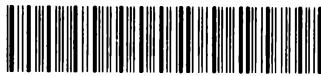
\includegraphics[keepaspectratio]{images/part004_82ba3e9c.jpg}}\\

